\documentclass{article}

\usepackage[%
    left=0.5in,%
    right=0.5in,%
    top=0.5in,%
    bottom=0.5in,%
]{geometry}%
\usepackage{minitoc}
\usepackage{multicol}
\usepackage{graphicx}
\usepackage{fixltx2e}
\usepackage{listings}
\usepackage{color}
\usepackage{hyperref}
    \hypersetup{ colorlinks = true, linkcolor = blue }
\usepackage{blindtext}
\definecolor{lightgray}{gray}{0.9}
\graphicspath{ {./} }

\newcommand{\inlinecode}[2]{\colorbox{lightgray}{\lstinline
[language=#1]$#2$}}
\newcommand{\worddef}[1]{\hyperref[sec:reference]{\textit{#1}}}

\begin{document}

\tableofcontents

\newpage

\section{IP security}
\begin{itemize}
  \item IP is connectionless and stateless
  \begin{itemize}
    \item Best effort service 
	  \item No delivery guarantee 
	  \item No order guarantee 
  \end{itemize}
	\item IPv4 No guaranteed security support 
	\item IPv6 security support is guaranteed - IPSec.
\end{itemize}

\subsection{IPSec}
\begin{itemize}
	\item Optional in IPv4, mandatory support in IPv6 
	\item Two major security mechanisms 
	\item IP Authentication Header (AH). (Not really used, because it's not to useful)
	\item IP Encapsulation Security Payload (EPS). We both encrypt and authenticate data
	\item Does not contain any mechanisms to prevent traffic analysis.
\end{itemize}

\section{Encapsulation Security Payload (ESP)}
\begin{flushleft}
Includes an additional header within the IP packet that describes what encryption and authentication is in use
\end{flushleft}
\begin{center}
  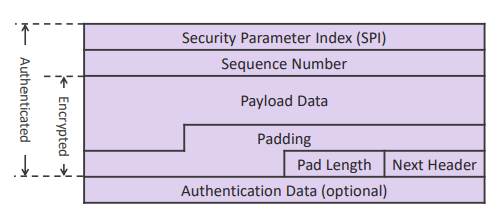
\includegraphics[scale=0.5]{esp_payload.png}
\end{center}

\subsection{Security parameter index}
\begin{itemize}
  \item Stores security parameters e.g. crypto protocol and keys 
  \item Established by Internet security association and key management protocol (ISAKMP) during the Internet Key Exchange (IKE) handshake 
  \item Uses Diffie-Hellman for key exchange 
  \item The SPI references the entry in a table that corresponds to this session’s parameters
\end{itemize}

\subsection{ESP in Transport Mode}
\begin{flushleft}
ESP uses either Transport or Tunnel modes
\end{flushleft}

\begin{center}
  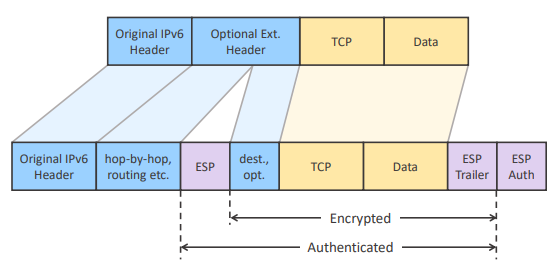
\includegraphics[scale=0.5]{esp_tunnel.png}
\end{center}

\subsection{ESP in tunnel mode}
\begin{center}
  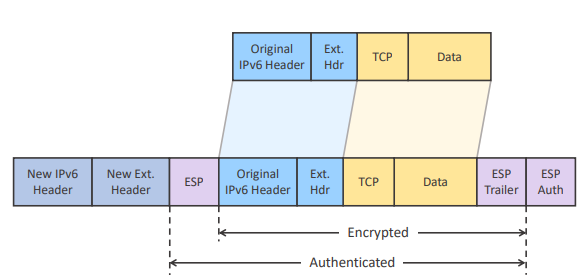
\includegraphics[scale=0.5]{esp_tunnel_.png}
\end{center}

\subsection{Transport vs tunnel modes}
\begin{itemize}
  \item \textbf{Transport mode} simply encrypts packets, providing \textbf{host-to-host encryption} but using the original header 
  \item Prevents contents being read, but doesn’t stop traffic analysis or manipulation of the header
  \item \textbf{Tunnel mode} (usually gateway-to-gateway) protects some segment of a channel with encryption 
  \item Provides some resistance to traffic analysis, and completely protects manipulation of the payload 
  \item VPNs are commonly implemented this way
\end{itemize}

\section{ARP}
\begin{itemize}
  \item ARP is a protocol used (in IPv4) to obtain physical MAC addresses for given IPs 
  \item It is used prior to constructing IP and TCP packets for communication 
  \item Network layer
  \item \textbf{ARP Cache Poisoning:} we can simply send an unrequested ARP reply, and overwrite the MAC address in a hosts ARP cache with our own
\end{itemize}

\subsection{ARP Protection}
\begin{itemize}
  \item Some OSs ignore \textbf{unsolicited ARP requests}, or can be configured to use ARP differently 
  \item Some software, such as intrusion detection packages, will include ARP spoofing detection 
  \item Maintain a log of current MAC:IP assignments and ARP requests / replies 
  \item Allows us to spot suspicious messages such as unsolicited ARP replies
\end{itemize}

\section{DNS}
\begin{itemize}
  \item DNS translates domain names into IP addresses. E.g. nottingham.ac.uk → 128.243.80.167 
  \item DNS packets are UDP. Stateless, on the transport layer 
  \item DNS resolvers \textbf{will cache} the IPs for a while
\end{itemize}

\subsection{DNS Spoofing}
\begin{itemize}
  \item If we can poison the cache of a nameserver people are using, we can replace a \textbf{website lookup with our IP}
  \item Can be achieved through prior arp cache poisoning, a reply flood or a Kaminsky attack
  \item \textbf{Kaminsky attack}: utilises the fact that cache restrainst, don't apply to sibling domains: (1.google.com, 2.google.com, etc.)
  \item Attackers can do this and say they’re the official server for www.google.com, telling the nameserver what www. needs to be, and the nameserver will believe the attacker.
\end{itemize}

\subsection{DNS protection}
\begin{itemize}
  \item Random query numbers help protect against spoof replies 
  \item Since the Kaminsky attack, most resolvers now randomise the source port too 
  \item DNSSEC aims to tackle DNS exploits by authenticating the name server and providing integrity for the messages
\end{itemize}

\section{Denial of Service Attacks}
\begin{itemize}
  \item A denial of service attack is an attempt to make a machine or network resource unavailable to its authorised / intended users 
  \item This will usually involve flooding a machine with enough requests that it can’t serve its legitimate purpose. E.g. Ping flood 
  \item A distributed denial of service occurs where there is more than one attacking machine
\end{itemize}

\subsection{TCP Syn Flooding}
\begin{itemize}
  \item Attacker initiates a genuine connection but then immediately breaks it 
  \item Attacker never finishes 3-way handshake 
  \item Victim is busy with the timeout 
  \item Attacker initiates large number of syn requests 
  \item Victim reaches its half-open connection limit 
  \item Denial of service
\end{itemize}

\section{Amplification Attacks}
\begin{itemize}
  \item Regular attacks are your bandwidth vs your targets 
  \item Amplification attacks utilise some aspect of a network protocol to increase the \textbf{bandwidth of an attack}
\end{itemize}

\subsection{Smurf and Fraggle Attacks}
\begin{itemize}
  \item Smurf attacks broadcast an ICMP Ping request to a router, but with a spoofed IP belonging to the victim 
  \item A Fraggle attack is identical in principle, using UDP echo packets
\end{itemize}
\begin{center}
  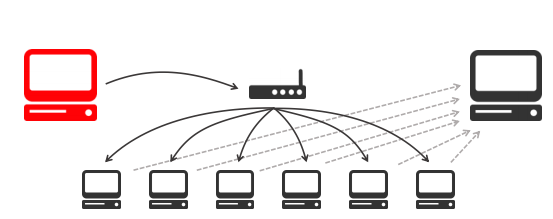
\includegraphics[scale=0.5]{smur.png}
\end{center}

\pagebreak

\subsection{DNS Amplification}
\begin{itemize}
  \item Recursive resolvers respond to DNS queries then return a response 
  \item This response can be many times larger than the query
  \item In an ideal world, all DNS resolvers would: 
  \item Use an authorised list of requesters – e.g. and ISP allowing requests from only their customers 
  \item Egress filtering – Why is this external IP using my resolver? 
  \item Many DNS servers are set up incorrectly, and will happily amplify your traffic – Open Resolvers 
  \item Botnets maintain lists of these open resolvers, and there are projects attempting to shut them down
\end{itemize}

\subsection{NTP Amplification}
\begin{itemize}
  \item NTP is a protocol for synchronising time between machines 
  \item Extremely similar to DNS amplification 
  \item \verb!MON_GETLIST! request returns the list of the last 600 contacts $\rightarrow$ 200x amplification
\end{itemize}

\section{Low and Slow}
\begin{itemize}
  \item \textbf{Slowloris} 
  \item Open numerous connections to a server 
  \item Begin an HTTP request, but never actually finish it 
  \item \textbf{R-U-Dead-Yet?} 
  \item Similar to slowloris 
  \item Begin an extremely long HTTP POST, send tiny amounts at a time
\end{itemize}

\pagebreak
\section*{Reference section} \label{sec:reference}
\begin{description}
	\item[placeholder] \hfill \\
\end{description}
\end{document}
